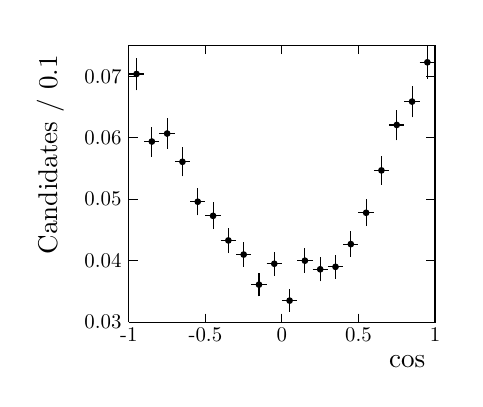
\begin{tikzpicture}
\pgfdeclareplotmark{cross} {
\pgfpathmoveto{\pgfpoint{-0.3\pgfplotmarksize}{\pgfplotmarksize}}
\pgfpathlineto{\pgfpoint{+0.3\pgfplotmarksize}{\pgfplotmarksize}}
\pgfpathlineto{\pgfpoint{+0.3\pgfplotmarksize}{0.3\pgfplotmarksize}}
\pgfpathlineto{\pgfpoint{+1\pgfplotmarksize}{0.3\pgfplotmarksize}}
\pgfpathlineto{\pgfpoint{+1\pgfplotmarksize}{-0.3\pgfplotmarksize}}
\pgfpathlineto{\pgfpoint{+0.3\pgfplotmarksize}{-0.3\pgfplotmarksize}}
\pgfpathlineto{\pgfpoint{+0.3\pgfplotmarksize}{-1.\pgfplotmarksize}}
\pgfpathlineto{\pgfpoint{-0.3\pgfplotmarksize}{-1.\pgfplotmarksize}}
\pgfpathlineto{\pgfpoint{-0.3\pgfplotmarksize}{-0.3\pgfplotmarksize}}
\pgfpathlineto{\pgfpoint{-1.\pgfplotmarksize}{-0.3\pgfplotmarksize}}
\pgfpathlineto{\pgfpoint{-1.\pgfplotmarksize}{0.3\pgfplotmarksize}}
\pgfpathlineto{\pgfpoint{-0.3\pgfplotmarksize}{0.3\pgfplotmarksize}}
\pgfpathclose
\pgfusepathqstroke
}
\pgfdeclareplotmark{cross*} {
\pgfpathmoveto{\pgfpoint{-0.3\pgfplotmarksize}{\pgfplotmarksize}}
\pgfpathlineto{\pgfpoint{+0.3\pgfplotmarksize}{\pgfplotmarksize}}
\pgfpathlineto{\pgfpoint{+0.3\pgfplotmarksize}{0.3\pgfplotmarksize}}
\pgfpathlineto{\pgfpoint{+1\pgfplotmarksize}{0.3\pgfplotmarksize}}
\pgfpathlineto{\pgfpoint{+1\pgfplotmarksize}{-0.3\pgfplotmarksize}}
\pgfpathlineto{\pgfpoint{+0.3\pgfplotmarksize}{-0.3\pgfplotmarksize}}
\pgfpathlineto{\pgfpoint{+0.3\pgfplotmarksize}{-1.\pgfplotmarksize}}
\pgfpathlineto{\pgfpoint{-0.3\pgfplotmarksize}{-1.\pgfplotmarksize}}
\pgfpathlineto{\pgfpoint{-0.3\pgfplotmarksize}{-0.3\pgfplotmarksize}}
\pgfpathlineto{\pgfpoint{-1.\pgfplotmarksize}{-0.3\pgfplotmarksize}}
\pgfpathlineto{\pgfpoint{-1.\pgfplotmarksize}{0.3\pgfplotmarksize}}
\pgfpathlineto{\pgfpoint{-0.3\pgfplotmarksize}{0.3\pgfplotmarksize}}
\pgfpathclose
\pgfusepathqfillstroke
}
\pgfdeclareplotmark{newstar} {
\pgfpathmoveto{\pgfqpoint{0pt}{\pgfplotmarksize}}
\pgfpathlineto{\pgfqpointpolar{44}{0.5\pgfplotmarksize}}
\pgfpathlineto{\pgfqpointpolar{18}{\pgfplotmarksize}}
\pgfpathlineto{\pgfqpointpolar{-20}{0.5\pgfplotmarksize}}
\pgfpathlineto{\pgfqpointpolar{-54}{\pgfplotmarksize}}
\pgfpathlineto{\pgfqpointpolar{-90}{0.5\pgfplotmarksize}}
\pgfpathlineto{\pgfqpointpolar{234}{\pgfplotmarksize}}
\pgfpathlineto{\pgfqpointpolar{198}{0.5\pgfplotmarksize}}
\pgfpathlineto{\pgfqpointpolar{162}{\pgfplotmarksize}}
\pgfpathlineto{\pgfqpointpolar{134}{0.5\pgfplotmarksize}}
\pgfpathclose
\pgfusepathqstroke
}
\pgfdeclareplotmark{newstar*} {
\pgfpathmoveto{\pgfqpoint{0pt}{\pgfplotmarksize}}
\pgfpathlineto{\pgfqpointpolar{44}{0.5\pgfplotmarksize}}
\pgfpathlineto{\pgfqpointpolar{18}{\pgfplotmarksize}}
\pgfpathlineto{\pgfqpointpolar{-20}{0.5\pgfplotmarksize}}
\pgfpathlineto{\pgfqpointpolar{-54}{\pgfplotmarksize}}
\pgfpathlineto{\pgfqpointpolar{-90}{0.5\pgfplotmarksize}}
\pgfpathlineto{\pgfqpointpolar{234}{\pgfplotmarksize}}
\pgfpathlineto{\pgfqpointpolar{198}{0.5\pgfplotmarksize}}
\pgfpathlineto{\pgfqpointpolar{162}{\pgfplotmarksize}}
\pgfpathlineto{\pgfqpointpolar{134}{0.5\pgfplotmarksize}}
\pgfpathclose
\pgfusepathqfillstroke
}
\definecolor{c}{rgb}{1,1,1};
\draw [color=c, fill=c] (0.1,0.0925676) rectangle (4.9,4.53581);
\draw [color=c, fill=c] (0.772,0.803486) rectangle (4.66,4.31365);
\definecolor{c}{rgb}{0,0,0};
\draw [c] (0.772,0.803486) -- (0.772,4.31365) -- (4.66,4.31365) -- (4.66,0.803486) -- (0.772,0.803486);
\draw [c,line width=0.4] (0.8692,3.74787) -- (0.8692,3.95483);
\draw [c,line width=0.4] (0.8692,3.95483) -- (0.8692,4.1618);
\draw [c,line width=0.4] (0.772,3.95483) -- (0.8692,3.95483);
\draw [c,line width=0.4] (0.8692,3.95483) -- (0.9664,3.95483);
\foreach \P in {(0.8692,3.95483)}{\draw[mark options={color=c,fill=c},mark size=1.201201pt,mark=*,mark size=1pt] plot coordinates {\P};}
\draw [c,line width=0.4] (1.0636,2.90668) -- (1.0636,3.09679);
\draw [c,line width=0.4] (1.0636,3.09679) -- (1.0636,3.2869);
\draw [c,line width=0.4] (0.9664,3.09679) -- (1.0636,3.09679);
\draw [c,line width=0.4] (1.0636,3.09679) -- (1.1608,3.09679);
\foreach \P in {(1.0636,3.09679)}{\draw[mark options={color=c,fill=c},mark size=1.201201pt,mark=*,mark size=1pt] plot coordinates {\P};}
\draw [c,line width=0.4] (1.258,3.00602) -- (1.258,3.1982);
\draw [c,line width=0.4] (1.258,3.1982) -- (1.258,3.39038);
\draw [c,line width=0.4] (1.1608,3.1982) -- (1.258,3.1982);
\draw [c,line width=0.4] (1.258,3.1982) -- (1.3552,3.1982);
\foreach \P in {(1.258,3.1982)}{\draw[mark options={color=c,fill=c},mark size=1.201201pt,mark=*,mark size=1pt] plot coordinates {\P};}
\draw [c,line width=0.4] (1.4524,2.65463) -- (1.4524,2.83938);
\draw [c,line width=0.4] (1.4524,2.83938) -- (1.4524,3.02414);
\draw [c,line width=0.4] (1.3552,2.83938) -- (1.4524,2.83938);
\draw [c,line width=0.4] (1.4524,2.83938) -- (1.5496,2.83938);
\foreach \P in {(1.4524,2.83938)}{\draw[mark options={color=c,fill=c},mark size=1.201201pt,mark=*,mark size=1pt] plot coordinates {\P};}
\draw [c,line width=0.4] (1.6468,2.15863) -- (1.6468,2.33236);
\draw [c,line width=0.4] (1.6468,2.33236) -- (1.6468,2.50608);
\draw [c,line width=0.4] (1.5496,2.33236) -- (1.6468,2.33236);
\draw [c,line width=0.4] (1.6468,2.33236) -- (1.744,2.33236);
\foreach \P in {(1.6468,2.33236)}{\draw[mark options={color=c,fill=c},mark size=1.201201pt,mark=*,mark size=1pt] plot coordinates {\P};}
\draw [c,line width=0.4] (1.8412,1.9833) -- (1.8412,2.15295);
\draw [c,line width=0.4] (1.8412,2.15295) -- (1.8412,2.3226);
\draw [c,line width=0.4] (1.744,2.15295) -- (1.8412,2.15295);
\draw [c,line width=0.4] (1.8412,2.15295) -- (1.9384,2.15295);
\foreach \P in {(1.8412,2.15295)}{\draw[mark options={color=c,fill=c},mark size=1.201201pt,mark=*,mark size=1pt] plot coordinates {\P};}
\draw [c,line width=0.4] (2.0356,1.67862) -- (2.0356,1.84093);
\draw [c,line width=0.4] (2.0356,1.84093) -- (2.0356,2.00325);
\draw [c,line width=0.4] (1.9384,1.84093) -- (2.0356,1.84093);
\draw [c,line width=0.4] (2.0356,1.84093) -- (2.1328,1.84093);
\foreach \P in {(2.0356,1.84093)}{\draw[mark options={color=c,fill=c},mark size=1.201201pt,mark=*,mark size=1pt] plot coordinates {\P};}
\draw [c,line width=0.4] (2.23,1.50358) -- (2.23,1.66153);
\draw [c,line width=0.4] (2.23,1.66153) -- (2.23,1.81947);
\draw [c,line width=0.4] (2.1328,1.66153) -- (2.23,1.66153);
\draw [c,line width=0.4] (2.23,1.66153) -- (2.3272,1.66153);
\foreach \P in {(2.23,1.66153)}{\draw[mark options={color=c,fill=c},mark size=1.201201pt,mark=*,mark size=1pt] plot coordinates {\P};}
\draw [c,line width=0.4] (2.4244,1.1311) -- (2.4244,1.27931);
\draw [c,line width=0.4] (2.4244,1.27931) -- (2.4244,1.42752);
\draw [c,line width=0.4] (2.3272,1.27931) -- (2.4244,1.27931);
\draw [c,line width=0.4] (2.4244,1.27931) -- (2.5216,1.27931);
\foreach \P in {(2.4244,1.27931)}{\draw[mark options={color=c,fill=c},mark size=1.201201pt,mark=*,mark size=1pt] plot coordinates {\P};}
\draw [c,line width=0.4] (2.6188,1.38949) -- (2.6188,1.54452);
\draw [c,line width=0.4] (2.6188,1.54452) -- (2.6188,1.69955);
\draw [c,line width=0.4] (2.5216,1.54452) -- (2.6188,1.54452);
\draw [c,line width=0.4] (2.6188,1.54452) -- (2.716,1.54452);
\foreach \P in {(2.6188,1.54452)}{\draw[mark options={color=c,fill=c},mark size=1.201201pt,mark=*,mark size=1pt] plot coordinates {\P};}
\draw [c,line width=0.4] (2.8132,0.933729) -- (2.8132,1.0765);
\draw [c,line width=0.4] (2.8132,1.0765) -- (2.8132,1.21927);
\draw [c,line width=0.4] (2.716,1.0765) -- (2.8132,1.0765);
\draw [c,line width=0.4] (2.8132,1.0765) -- (2.9104,1.0765);
\foreach \P in {(2.8132,1.0765)}{\draw[mark options={color=c,fill=c},mark size=1.201201pt,mark=*,mark size=1pt] plot coordinates {\P};}
\draw [c,line width=0.4] (3.0076,1.42752) -- (3.0076,1.58352);
\draw [c,line width=0.4] (3.0076,1.58352) -- (3.0076,1.73953);
\draw [c,line width=0.4] (2.9104,1.58352) -- (3.0076,1.58352);
\draw [c,line width=0.4] (3.0076,1.58352) -- (3.1048,1.58352);
\foreach \P in {(3.0076,1.58352)}{\draw[mark options={color=c,fill=c},mark size=1.201201pt,mark=*,mark size=1pt] plot coordinates {\P};}
\draw [c,line width=0.4] (3.202,1.32106) -- (3.202,1.47432);
\draw [c,line width=0.4] (3.202,1.47432) -- (3.202,1.62757);
\draw [c,line width=0.4] (3.1048,1.47432) -- (3.202,1.47432);
\draw [c,line width=0.4] (3.202,1.47432) -- (3.2992,1.47432);
\foreach \P in {(3.202,1.47432)}{\draw[mark options={color=c,fill=c},mark size=1.201201pt,mark=*,mark size=1pt] plot coordinates {\P};}
\draw [c,line width=0.4] (3.3964,1.35147) -- (3.3964,1.50552);
\draw [c,line width=0.4] (3.3964,1.50552) -- (3.3964,1.65956);
\draw [c,line width=0.4] (3.2992,1.50552) -- (3.3964,1.50552);
\draw [c,line width=0.4] (3.3964,1.50552) -- (3.4936,1.50552);
\foreach \P in {(3.3964,1.50552)}{\draw[mark options={color=c,fill=c},mark size=1.201201pt,mark=*,mark size=1pt] plot coordinates {\P};}
\draw [c,line width=0.4] (3.5908,1.63295) -- (3.5908,1.79413);
\draw [c,line width=0.4] (3.5908,1.79413) -- (3.5908,1.95532);
\draw [c,line width=0.4] (3.4936,1.79413) -- (3.5908,1.79413);
\draw [c,line width=0.4] (3.5908,1.79413) -- (3.688,1.79413);
\foreach \P in {(3.5908,1.79413)}{\draw[mark options={color=c,fill=c},mark size=1.201201pt,mark=*,mark size=1pt] plot coordinates {\P};}
\draw [c,line width=0.4] (3.7852,2.02141) -- (3.7852,2.19195);
\draw [c,line width=0.4] (3.7852,2.19195) -- (3.7852,2.36249);
\draw [c,line width=0.4] (3.688,2.19195) -- (3.7852,2.19195);
\draw [c,line width=0.4] (3.7852,2.19195) -- (3.8824,2.19195);
\foreach \P in {(3.7852,2.19195)}{\draw[mark options={color=c,fill=c},mark size=1.201201pt,mark=*,mark size=1pt] plot coordinates {\P};}
\draw [c,line width=0.4] (3.9796,2.54774) -- (3.9796,2.73018);
\draw [c,line width=0.4] (3.9796,2.73018) -- (3.9796,2.91261);
\draw [c,line width=0.4] (3.8824,2.73018) -- (3.9796,2.73018);
\draw [c,line width=0.4] (3.9796,2.73018) -- (4.0768,2.73018);
\foreach \P in {(3.9796,2.73018)}{\draw[mark options={color=c,fill=c},mark size=1.201201pt,mark=*,mark size=1pt] plot coordinates {\P};}
\draw [c,line width=0.4] (4.174,3.11302) -- (4.174,3.3074);
\draw [c,line width=0.4] (4.174,3.3074) -- (4.174,3.50179);
\draw [c,line width=0.4] (4.0768,3.3074) -- (4.174,3.3074);
\draw [c,line width=0.4] (4.174,3.3074) -- (4.2712,3.3074);
\foreach \P in {(4.174,3.3074)}{\draw[mark options={color=c,fill=c},mark size=1.201201pt,mark=*,mark size=1pt] plot coordinates {\P};}
\draw [c,line width=0.4] (4.3684,3.40357) -- (4.3684,3.60382);
\draw [c,line width=0.4] (4.3684,3.60382) -- (4.3684,3.80406);
\draw [c,line width=0.4] (4.2712,3.60382) -- (4.3684,3.60382);
\draw [c,line width=0.4] (4.3684,3.60382) -- (4.4656,3.60382);
\foreach \P in {(4.3684,3.60382)}{\draw[mark options={color=c,fill=c},mark size=1.201201pt,mark=*,mark size=1pt] plot coordinates {\P};}
\draw [c,line width=0.4] (4.5628,3.8933) -- (4.5628,4.10304);
\draw [c,line width=0.4] (4.5628,4.10304) -- (4.5628,4.31278);
\draw [c,line width=0.4] (4.4656,4.10304) -- (4.5628,4.10304);
\draw [c,line width=0.4] (4.5628,4.10304) -- (4.66,4.10304);
\foreach \P in {(4.5628,4.10304)}{\draw[mark options={color=c,fill=c},mark size=1.201201pt,mark=*,mark size=1pt] plot coordinates {\P};}
\draw [c,line width=0.4] (0.772,0.803486) -- (4.66,0.803486);
\draw [anchor= east] (4.66,0.305843) node[scale=0.979298, rotate=0]{$\cos\thetaK$};
\draw [c,line width=0.4] (0.772,0.911457) -- (0.772,0.803486);
\draw [c,line width=0.4] (1.744,0.911457) -- (1.744,0.803486);
\draw [c,line width=0.4] (2.716,0.911457) -- (2.716,0.803486);
\draw [c,line width=0.4] (3.688,0.911457) -- (3.688,0.803486);
\draw [c,line width=0.4] (4.66,0.911457) -- (4.66,0.803486);
\draw [anchor=base] (0.772,0.563551) node[scale=0.753306, rotate=0]{-1};
\draw [anchor=base] (1.744,0.563551) node[scale=0.753306, rotate=0]{-0.5};
\draw [anchor=base] (2.716,0.563551) node[scale=0.753306, rotate=0]{0};
\draw [anchor=base] (3.688,0.563551) node[scale=0.753306, rotate=0]{0.5};
\draw [anchor=base] (4.66,0.563551) node[scale=0.753306, rotate=0]{1};
\draw [c,line width=0.4] (0.772,4.31365) -- (4.66,4.31365);
\draw [c,line width=0.4] (0.772,4.20568) -- (0.772,4.31365);
\draw [c,line width=0.4] (1.744,4.20568) -- (1.744,4.31365);
\draw [c,line width=0.4] (2.716,4.20568) -- (2.716,4.31365);
\draw [c,line width=0.4] (3.688,4.20568) -- (3.688,4.31365);
\draw [c,line width=0.4] (4.66,4.20568) -- (4.66,4.31365);
\draw [c,line width=0.4] (0.772,0.803486) -- (0.772,4.31365);
\draw [anchor= east] (-0.2264,4.31365) node[scale=0.979298, rotate=90]{Candidates / 0.1};
\draw [c,line width=0.4] (0.88576,0.803486) -- (0.772,0.803486);
\draw [c,line width=0.4] (0.88576,1.58352) -- (0.772,1.58352);
\draw [c,line width=0.4] (0.88576,2.36356) -- (0.772,2.36356);
\draw [c,line width=0.4] (0.88576,3.14359) -- (0.772,3.14359);
\draw [c,line width=0.4] (0.88576,3.92363) -- (0.772,3.92363);
\draw [c,line width=0.4] (0.88576,3.92363) -- (0.772,3.92363);
\draw [anchor= east] (0.772,0.803486) node[scale=0.753306, rotate=0]{0.03};
\draw [anchor= east] (0.772,1.58352) node[scale=0.753306, rotate=0]{0.04};
\draw [anchor= east] (0.772,2.36356) node[scale=0.753306, rotate=0]{0.05};
\draw [anchor= east] (0.772,3.14359) node[scale=0.753306, rotate=0]{0.06};
\draw [anchor= east] (0.772,3.92363) node[scale=0.753306, rotate=0]{0.07};
\draw [c,line width=0.4] (4.66,0.803486) -- (4.66,4.31365);
\draw [c,line width=0.4] (4.54624,0.803486) -- (4.66,0.803486);
\draw [c,line width=0.4] (4.54624,1.58352) -- (4.66,1.58352);
\draw [c,line width=0.4] (4.54624,2.36356) -- (4.66,2.36356);
\draw [c,line width=0.4] (4.54624,3.14359) -- (4.66,3.14359);
\draw [c,line width=0.4] (4.54624,3.92363) -- (4.66,3.92363);
\draw [c,line width=0.4] (4.54624,3.92363) -- (4.66,3.92363);
\end{tikzpicture}
